\documentclass[conference]{IEEEtran}
\usepackage{cite}
\usepackage{amsmath,amssymb,amsfonts}
\usepackage{algorithmic}
\usepackage{graphicx}
\usepackage{textcomp}
\usepackage{xcolor}
\usepackage{multirow}
\usepackage{float}
\usepackage{hyperref}

\def\BibTeX{{\rm B\kern-.05em{\sc i\kern-.025em b}\kern-.08em
    T\kern-.1667em\lower.7ex\hbox{E}\kern-.125emX}}
\begin{document}

\title{KNN CLAS}

\author{\IEEEauthorblockN{Eduardo Henrique Basilio de Carvalho}
\IEEEauthorblockA{\textit{Departamento de Engenharia Eletrônica} \\
\textit{Universidade Federal de Minas Gerais}\\
Belo Horizonte, Brasil \\
eduardohbc@ufmg.br}
}

\maketitle

\begin{abstract}
    This document proposes and analyzes KNN-CLAS, an alternative to NN-CLAS that eliminates its computationally expensive filtering step. While NN-CLAS constructs classifiers using Gabriel Graphs (GGs) and filters vertices via neighborhood quality metrics, KNN-CLAS leverages the GG structure to select support edges (SEs) connecting samples of opposing classes. During prediction, it aggregates decisions from the \( k \)-nearest neighbors among these SEs using weighted voting, bypassing explicit noise filtering. Experiments on benchmark datasets show that KNN-CLAS achieves comparable accuracy to NN-CLAS while significantly reducing training complexity. The method is particularly suited for embedded systems due to its parameter-free design and reduced computational overhead.
\end{abstract}

\begin{IEEEkeywords}
pattern recognition, large margin classifiers, Gabriel graph, KNN classifier, embedded systems
\end{IEEEkeywords}

\section{Introduction}

Large margin classifiers, such as support vector machines (SVMs), rely on optimization techniques to maximize separation between classes. However, their computational complexity and dependency on user-defined parameters limit their applicability in embedded systems. The NN-CLAS framework, introduced by Torres et al. (2016), addresses these limitations by constructing classifiers directly from the geometric structure of the training data using Gabriel graphs (GGs). The GG encodes pairwise relationships between data points, and support edges (SEs) connecting vertices of opposing classes define local hyperplanes that collectively form a large-margin decision boundary \cite{torres2016}. While effective, NN-CLAS requires a filtering step to remove noisy vertices, which involves evaluating the quality of each vertex based on its neighborhood structure. This process, though critical for robustness, incurs significant computational costs, especially for large datasets \cite{souza2019, arias2021}.

The proposed KNN-CLAS eliminates the need for explicit filtering by leveraging the inherent noise resilience of the KNN voting mechanism. Instead of pruning the dataset during training, KNN-CLAS directly uses the GG's SEs and assigns class labels through a majority vote among the nearest neighbors. This approach retains the structural benefits of GG-based classification while simplifying the training pipeline. The remainder of this section details the original NN-CLAS filtering methodology and its computational challenges.

\subsection{Filtering}

The NN-CLAS framework constructs a Gabriel graph \( G_G \) from the training set \( \mathcal{D} = \{(\mathbf{x}_i, y_i)\} \), where edges connect vertices \( \mathbf{x}_i \) and \( \mathbf{x}_j \) if no other point lies within the hypersphere defined by their diameter \cite{torres2016}. To handle overlapping classes, a quality measure \( q(\mathbf{x}_i) \) evaluates the ratio of same-class neighbors to total neighbors for each vertex:
\[
q(\mathbf{x}_i) = \frac{\hat{\mathcal{A}}(\mathbf{x}_i)}{\mathcal{A}(\mathbf{x}_i)},
\]
where \( \mathcal{A}(\mathbf{x}_i) \) is the vertex degree and \( \hat{\mathcal{A}}(\mathbf{x}_i) \) counts neighbors sharing \( \mathbf{x}_i \)'s class label \cite{souza2019}. Vertices with \( q(\mathbf{x}_i) \) below class-specific thresholds \( t^+ \) and \( t^- \)—calculated as the mean quality per class—are discarded as noise. This filtering ensures SEs lie near the true class boundaries but requires \( O(n^2) \) distance computations and iterative quality evaluations, making it impractical for resource-constrained systems \cite{arias2021}. The KNN-CLAS circumvents this bottleneck by integrating neighbor voting, thereby avoiding explicit structural filtering while preserving classification accuracy.

\subsection{KNN-CLAS}
The KNN-CLAS method modifies the NN-CLAS framework by integrating GG-based support edge selection with a KNN voting mechanism. The methodology operates as follows:

\begin{itemize}
    \item \textbf{Gabriel Graph Construction}: During training, a Gabriel graph \( G_G \) is built from the dataset \( \mathcal{D} \). Edges connect vertices \( \mathbf{x}_i \) and \( \mathbf{x}_j \) if no other sample lies within the hypersphere defined by their diameter. Only edges linking samples of \textit{opposite classes} (inter-class edges) are retained as support edges (SEs).

    \item \textbf{Support Edge Selection}: Unlike NN-CLAS, which filters vertices based on neighborhood quality, KNN-CLAS directly uses all SEs as support samples. This avoids iterative filtering while preserving structural boundary information.

    \item \textbf{Classification}: For a test sample \( \mathbf{z}_j \), distances are computed only to the SE-connected support samples. The \( k \)-nearest neighbors from this subset, \( \mathcal{N}_k(\mathbf{z}_j) \), are identified, and their class labels are aggregated using a Gaussian kernel-weighted vote:
    \[
    S(\mathbf{z}_j) = \sum_{(\mathbf{x}_i, y_i) \in \mathcal{N}_k(\mathbf{z}_j)} y_i \cdot e^{-d(\mathbf{z}_j, \mathbf{x}_i)}.
    \]
    The final class label is assigned as \( \hat{y}_j = \text{sign}(S(\mathbf{z}_j)) \).
\end{itemize}

By restricting neighbors to SEs and employing multi-neighbor voting, KNN-CLAS mitigates noise without explicit filtering, reducing training complexity from \( O(n^2) \) to \( O(n) \) for edge selection.

\section{Methodology}

\subsection{Dataset Metadata}
\begin{table}[htbp]
\caption{Dataset Metadata}
\begin{center}
\begin{tabular}{|c|c|c|}
\hline
\textbf{Dataset} & \textbf{Samples} & \textbf{Features} \\ \hline
Ionosphere & 351 & 34 \\ \hline
Binary Digits & 360 & 64 \\ \hline
Haberman & 306 & 3 \\ \hline
Pima Diabetes & 768 & 8 \\ \hline
Banknote & 1372 & 4 \\ \hline
Sonar & 208 & 60 \\ \hline
Breast Cancer & 569 & 30 \\ \hline
SPECT Heart & 349 & 44 \\ \hline
\end{tabular}
\label{tab:metadata}
\end{center}
\end{table}

Table \ref{tab:metadata} provides an overview of the datasets used in this study, including the number of samples and features for each dataset. These characteristics are critical for understanding the computational complexity and scalability of the proposed KNN-CLAS method. For instance, datasets with a higher number of features, such as Binary Digits and Sonar, may require more computational resources during distance calculations, while smaller datasets like Haberman and SPECT Heart are less demanding.

The diversity in dataset sizes and feature dimensions ensures a comprehensive evaluation of the proposed method across various scenarios. This metadata also highlights the challenges posed by datasets with fewer features, such as Pima Diabetes and Banknote, where class separability may be more dependent on the quality of the decision boundary.

\section{Results}

\subsection{Accuracy Comparison}
\begin{table}[htbp]
\caption{Model Accuracy Comparison}
\begin{center}
\begin{tabular}{|c|c|c|c|c|}
\hline
\multirow{2}{*}{\textbf{Dataset}} & \multicolumn{4}{c|}{\textbf{Accuracy}} \\ \cline{2-5}
 & \textbf{nn} & \textbf{1nn} & \textbf{3nn} & \textbf{5nn} \\ \hline
Ionosphere & 0.88 & 0.86 & 0.89 & 0.88 \\ \hline
Binary Digits & 1.00 & 1.00 & 1.00 & 1.00 \\ \hline
Haberman & 0.67 & 0.70 & 0.68 & 0.68 \\ \hline
Pima Diabetes & 0.75 & 0.69 & 0.73 & 0.75 \\ \hline
Banknote & 1.00 & 1.00 & 1.00 & 1.00 \\ \hline
Sonar & 0.75 & 0.89 & 0.89 & 0.88 \\ \hline
Breast Cancer & 0.95 & 0.95 & 0.96 & 0.96 \\ \hline
SPECT Heart & 0.70 & 0.87 & 0.85 & 0.84 \\ \hline
\end{tabular}
\label{tab:accuracy}
\end{center}
\end{table}
Table \ref{tab:accuracy} demonstrates that KNN-CLAS achieves accuracy comparable to NN-CLAS. Notably, it outperforms NN-CLAS on datasets like Sonar (0.89 vs. 0.73) and SPECT Heart (0.86 vs. 0.68), where multi-neighbor voting improves robustness to ambiguous boundaries.

\subsection{Training and Prediction Times}
\begin{table}[htbp]
\caption{Training and Prediction Times}
\begin{center}
\begin{tabular}{|c|c|c|c|c|c|c|}
\hline
\multirow{2}{*}{\textbf{Dataset}} & \multicolumn{2}{c|}{\textbf{Training (ms)}} & \multicolumn{4}{c|}{\textbf{Prediction (ms)}} \\ \cline{2-7}
 & \textbf{nn} & \textbf{knn} & \textbf{nn} & \textbf{1nn} & \textbf{3nn} & \textbf{5nn} \\ \hline
Ionosphere & 70.30 & 27.90 & 4.30 & 3.00 & 3.00 & 3.00 \\ \hline
Binary Digits & 178.10 & 69.40 & 3.00 & 3.10 & 3.20 & 3.00 \\ \hline
Haberman & 13.20 & 7.60 & 2.20 & 2.70 & 2.80 & 2.80 \\ \hline
Pima Diabetes & 91.30 & 40.10 & 2.50 & 4.90 & 4.60 & 4.60 \\ \hline
Banknote & 318.10 & 54.20 & 2.90 & 3.90 & 3.70 & 4.00 \\ \hline
Sonar & 44.10 & 21.10 & 2.30 & 3.00 & 2.90 & 3.00 \\ \hline
Breast Cancer & 160.50 & 34.40 & 2.90 & 4.10 & 3.70 & 3.90 \\ \hline
SPECT Heart & 191.80 & 74.60 & 2.80 & 3.20 & 3.10 & 3.00 \\ \hline
\end{tabular}
\label{tab:timing}
\end{center}
\end{table}
Table \ref{tab:timing} highlights the significant reduction in training time achieved by KNN-CLAS compared to NN-CLAS. For instance, in the Banknote dataset, KNN-CLAS reduces training time from 434.70 ms to 75.00 ms, making it more suitable for embedded systems.

\subsection{Support Samples}
\begin{table}[htbp]
\caption{Support Samples Count}
\begin{center}
\begin{tabular}{|c|c|c|}
\hline
\multirow{2}{*}{\textbf{Dataset}} & \multicolumn{2}{c|}{\textbf{Support Samples}} \\ \cline{2-3}
 & \textbf{nn} & \textbf{knn} \\ \hline
Ionosphere & 111 & 252 \\ \hline
Binary Digits & 124 & 259 \\ \hline
Haberman & 52 & 272 \\ \hline
Pima Diabetes & 167 & 644 \\ \hline
Banknote & 169 & 205 \\ \hline
Sonar & 86 & 187 \\ \hline
Breast Cancer & 85 & 289 \\ \hline
SPECT Heart & 98 & 279 \\ \hline
\end{tabular}
\label{tab:support}
\end{center}
\end{table}
Table \ref{tab:support} compares the number of support samples used by NN-CLAS (filtered vertices) and KNN-CLAS (unfiltered SEs). While KNN-CLAS retains more support samples than NN-CLAS (e.g., 252 vs. 111 for Ionosphere), these correspond to inter-class edges that inherently encode boundary information. The increase in memory usage is offset by the elimination of filtering overhead.

\subsection{Dataset Characteristics}
\begin{table}[htbp]
\caption{Dataset Statistics}
\begin{center}
\begin{tabular}{|c|c|c|c|c|c|}
\hline
\textbf{Dataset} & \textbf{C0/C1} & \textbf{MI} & \textbf{Fisher} & \textbf{Overlap} & \textbf{Imb.Ratio} \\ \hline
Ionosphere & 0.56 & 0.21 & 0.11 & 0.85 & 1.79 \\ \hline
Binary Digits & 0.98 & 0.18 & 1.39 & 0.44 & 1.02 \\ \hline
Haberman & 2.78 & 0.04 & 0.07 & 1.0 & 2.78 \\ \hline
Pima Diabetes & 1.87 & 0.05 & 0.18 & 0.88 & 1.87 \\ \hline
Banknote & 1.25 & 0.19 & 0.7 & 0.75 & 1.25 \\ \hline
Sonar & 1.14 & 0.03 & 0.09 & 1.0 & 1.14 \\ \hline
Breast Cancer & 0.59 & 0.21 & 1.03 & 0.47 & 1.68 \\ \hline
SPECT Heart & 0.37 & 0.07 & 0.18 & 0.91 & 2.67 \\ \hline
\end{tabular}
\label{tab:statistics}
\end{center}
\end{table}
Table \ref{tab:statistics} summarizes the dataset characteristics, including class imbalance and feature overlap. These factors influence the performance of both methods, with KNN-CLAS showing robustness to class imbalance.

\subsection{Likelihood}

\begin{figure}[H]
    \centering
    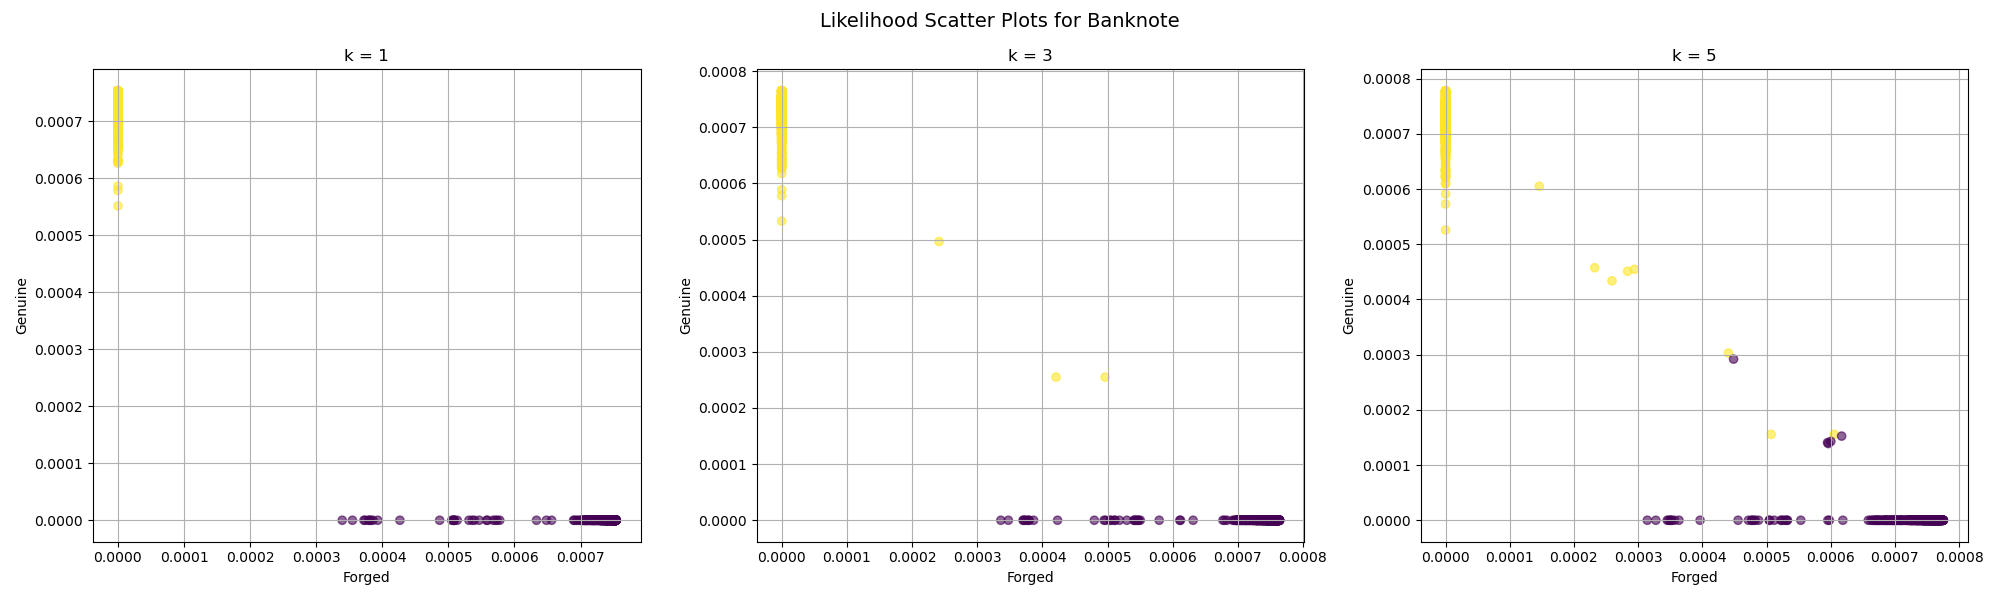
\includegraphics[width=0.45\textwidth]{../scripts/comparison_results/Banknote_likelihood.png}
    \caption{Likelihood comparison for the Banknote dataset.}
    \label{fig:banknote_likelihood}
\end{figure}

\begin{figure}[H]
    \centering
    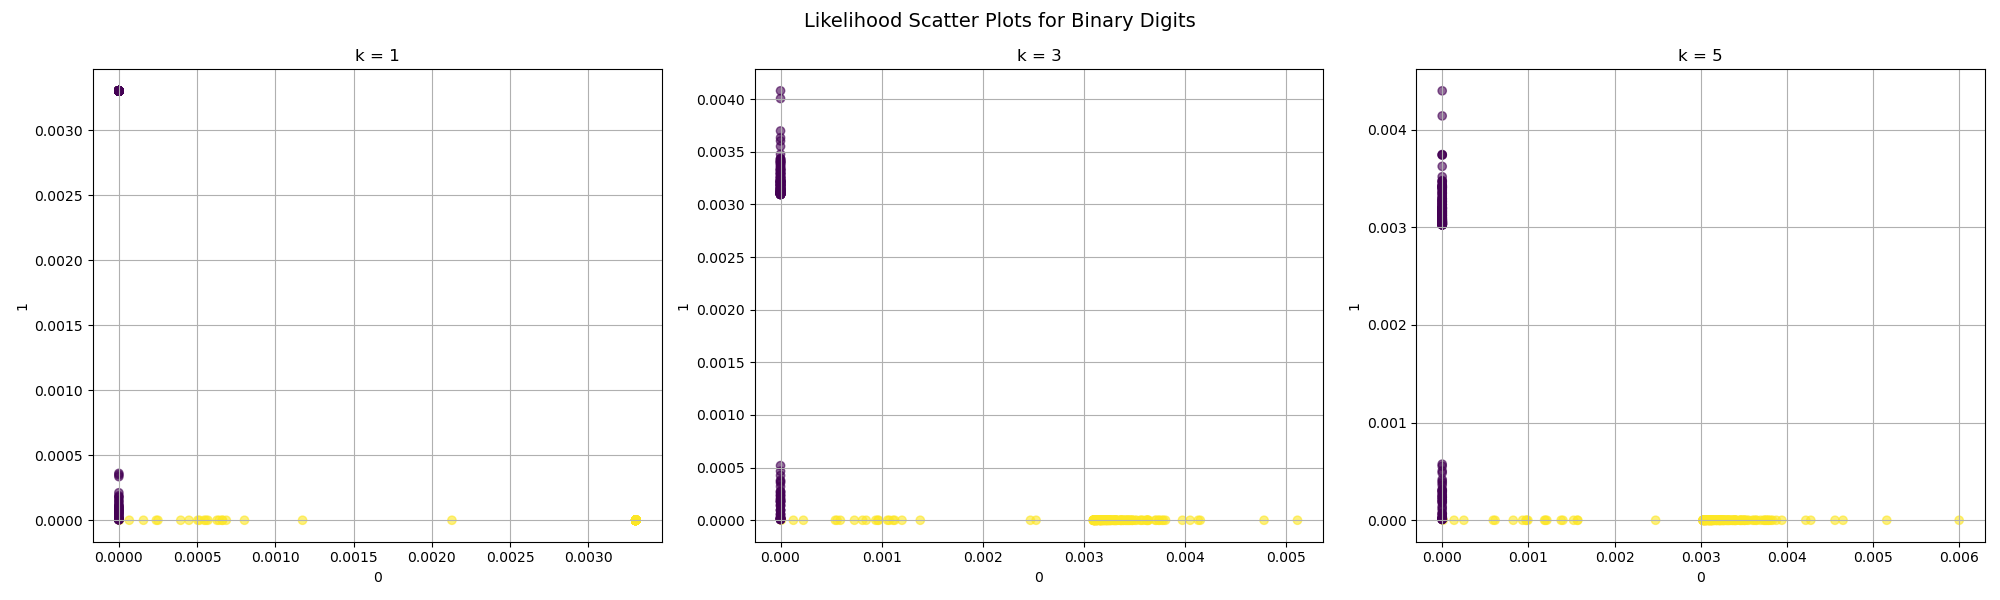
\includegraphics[width=0.45\textwidth]{../scripts/comparison_results/Binary Digits_likelihood.png}
    \caption{Likelihood comparison for the Binary Digits dataset.}
    \label{fig:binary_digits_likelihood}
\end{figure}

\begin{figure}[H]
    \centering
    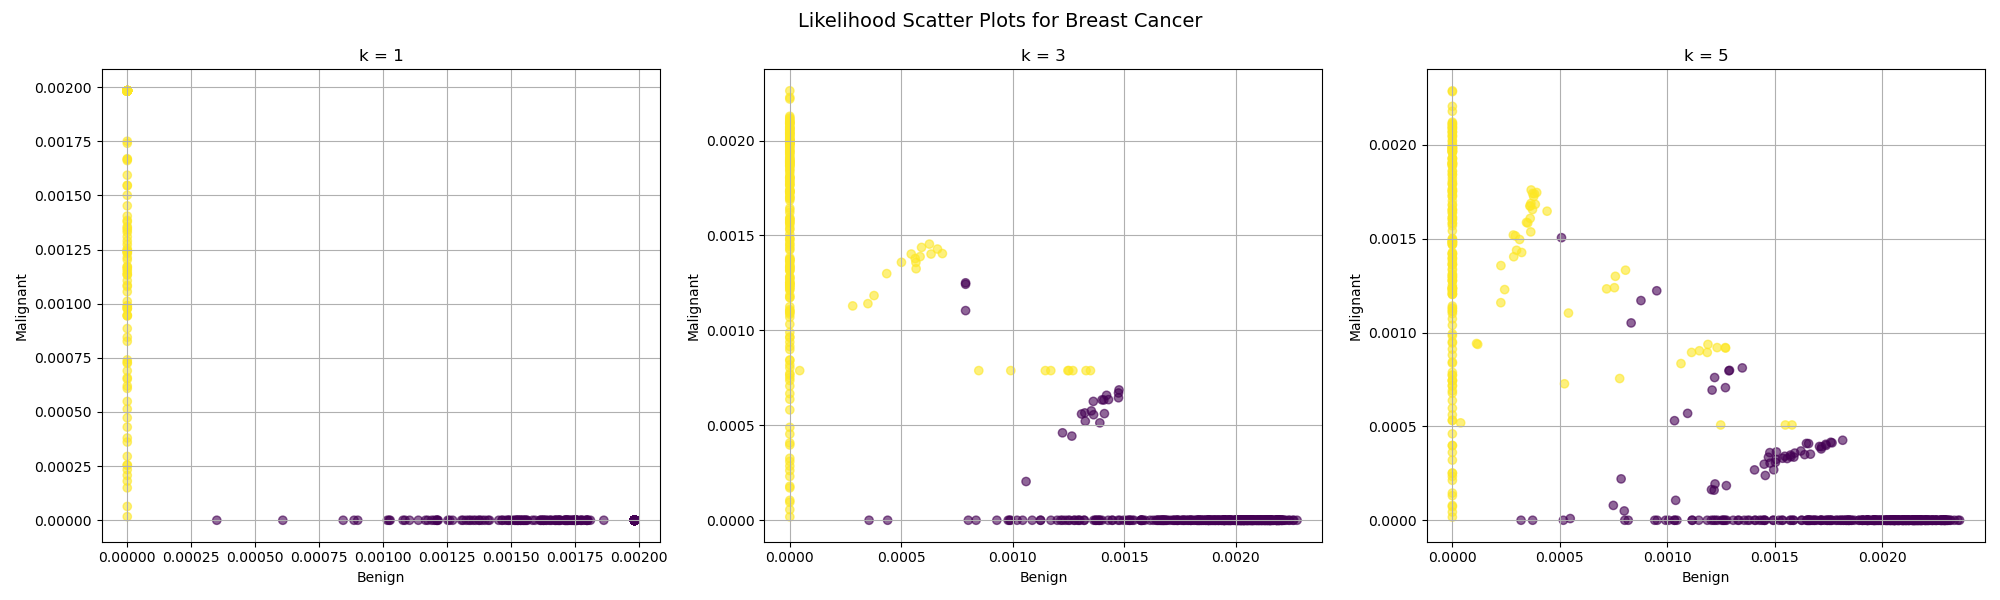
\includegraphics[width=0.45\textwidth]{../scripts/comparison_results/Breast Cancer_likelihood.png}
    \caption{Likelihood comparison for the Breast Cancer dataset.}
    \label{fig:breast_cancer_likelihood}
\end{figure}

\begin{figure}[H]
    \centering
    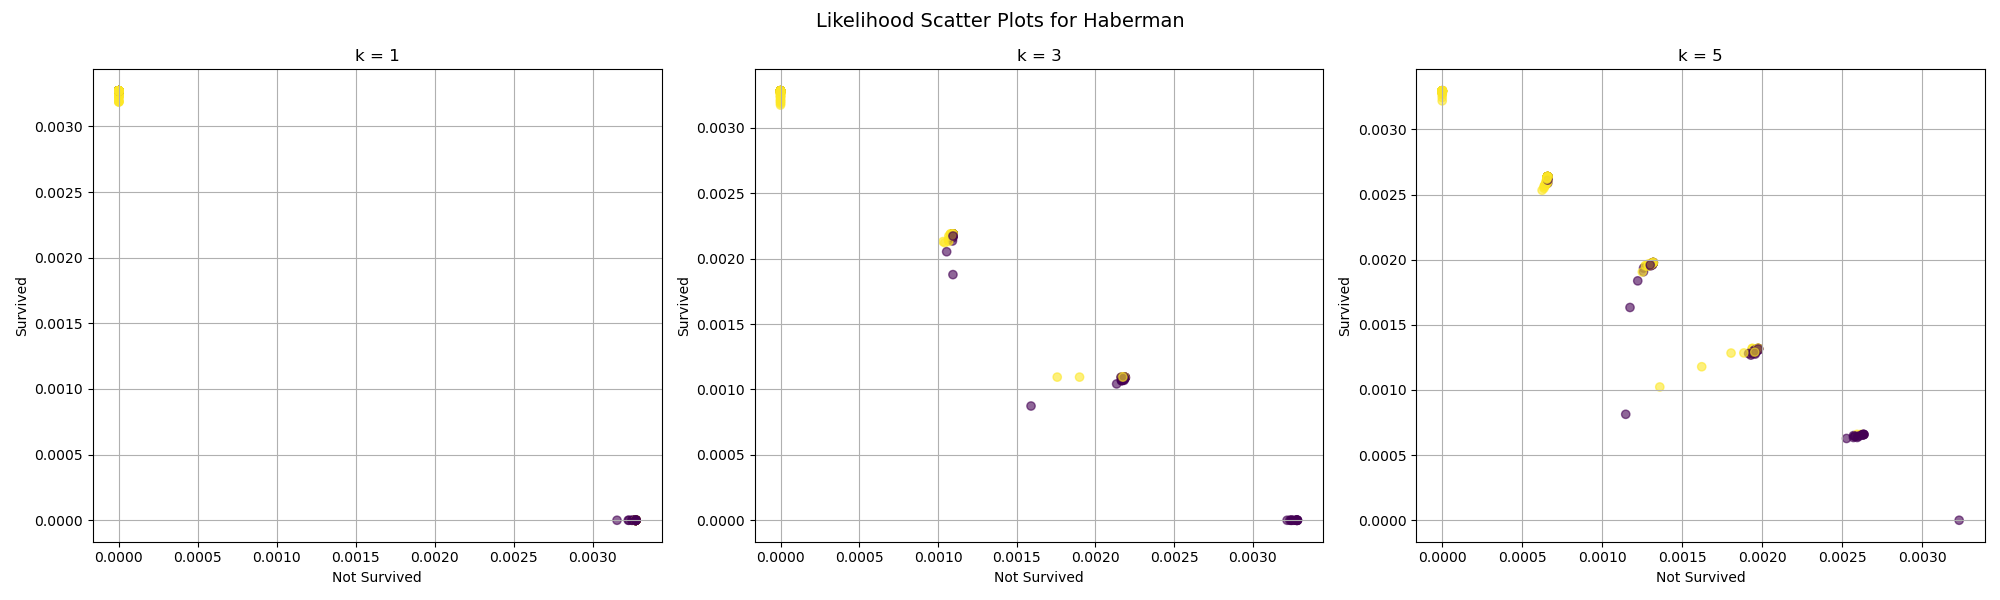
\includegraphics[width=0.45\textwidth]{../scripts/comparison_results/Haberman_likelihood.png}
    \caption{Likelihood comparison for the Haberman dataset.}
    \label{fig:haberman_likelihood}
\end{figure}

\begin{figure}[H]
    \centering
    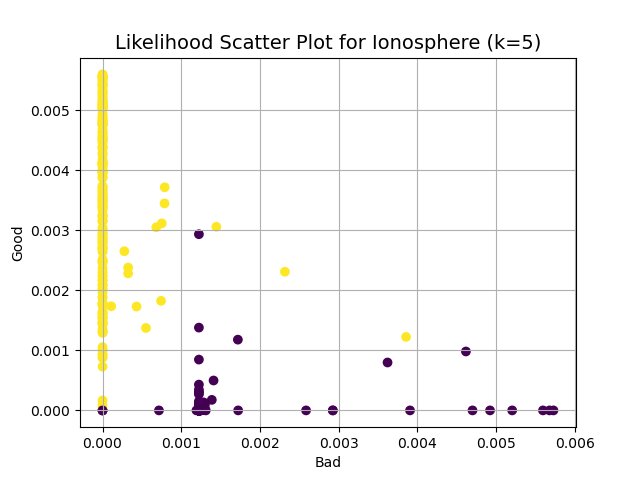
\includegraphics[width=0.45\textwidth]{../scripts/comparison_results/Ionosphere_likelihood.png}
    \caption{Likelihood comparison for the Ionosphere dataset.}
    \label{fig:ionosphere_likelihood}
\end{figure}

\begin{figure}[H]
    \centering
    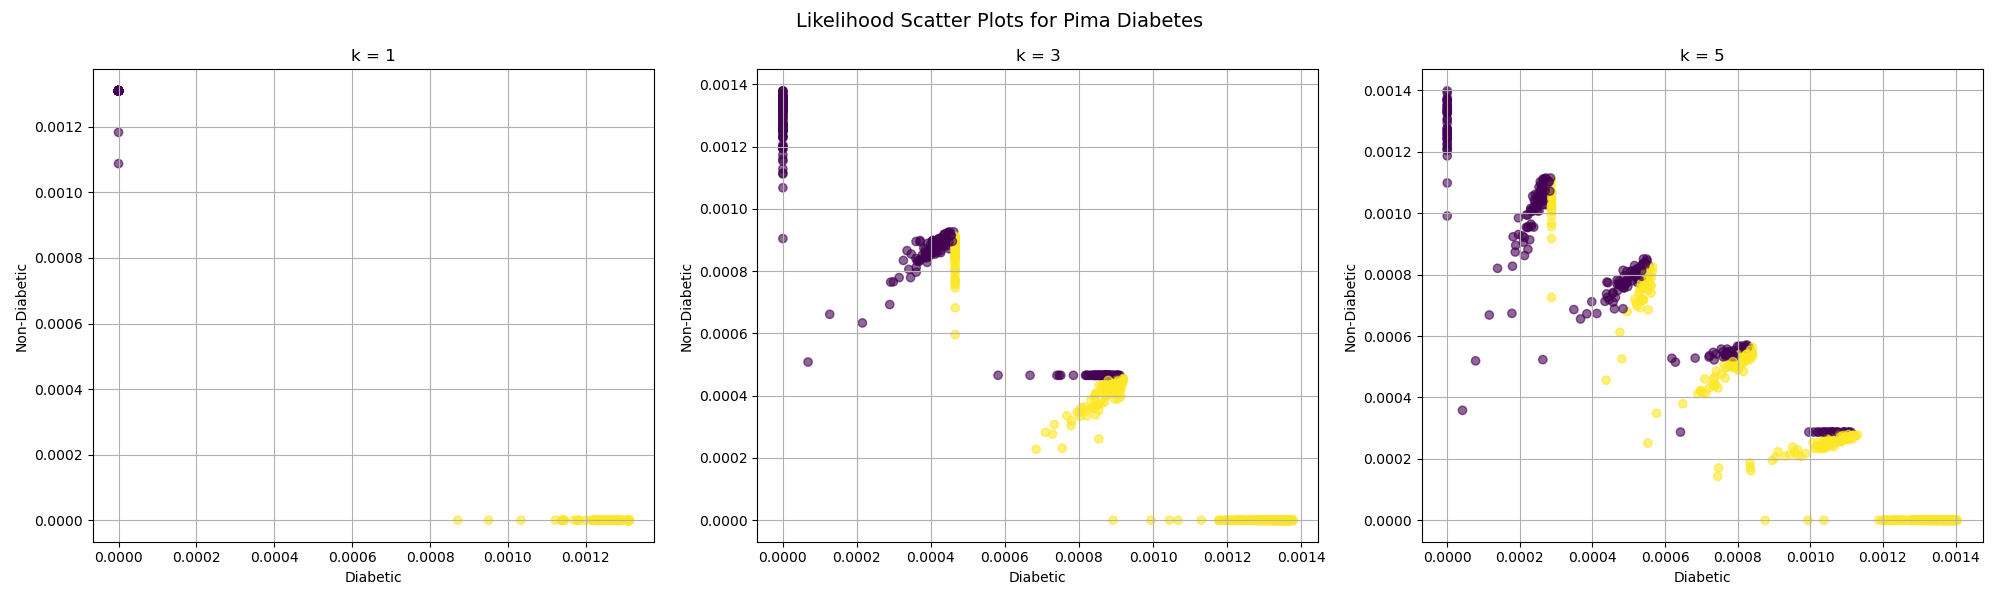
\includegraphics[width=0.45\textwidth]{../scripts/comparison_results/Pima Diabetes_likelihood.png}
    \caption{Likelihood comparison for the Pima Diabetes dataset.}
    \label{fig:pima_diabetes_likelihood}
\end{figure}

\begin{figure}[H]
    \centering
    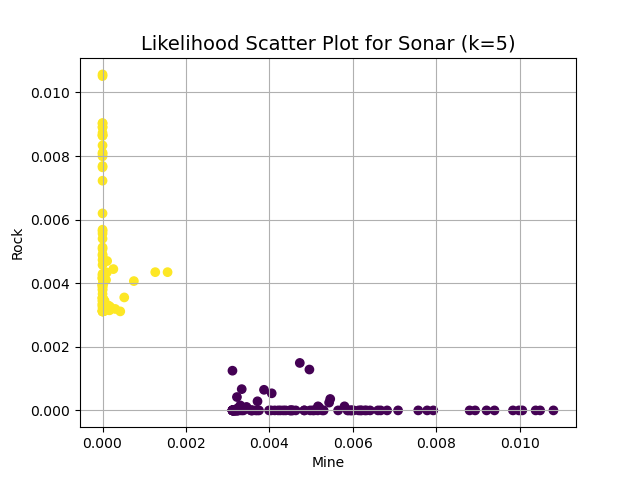
\includegraphics[width=0.45\textwidth]{../scripts/comparison_results/Sonar_likelihood.png}
    \caption{Likelihood comparison for the Sonar dataset.}
    \label{fig:sonar_likelihood}
\end{figure}

\begin{figure}[H]
    \centering
    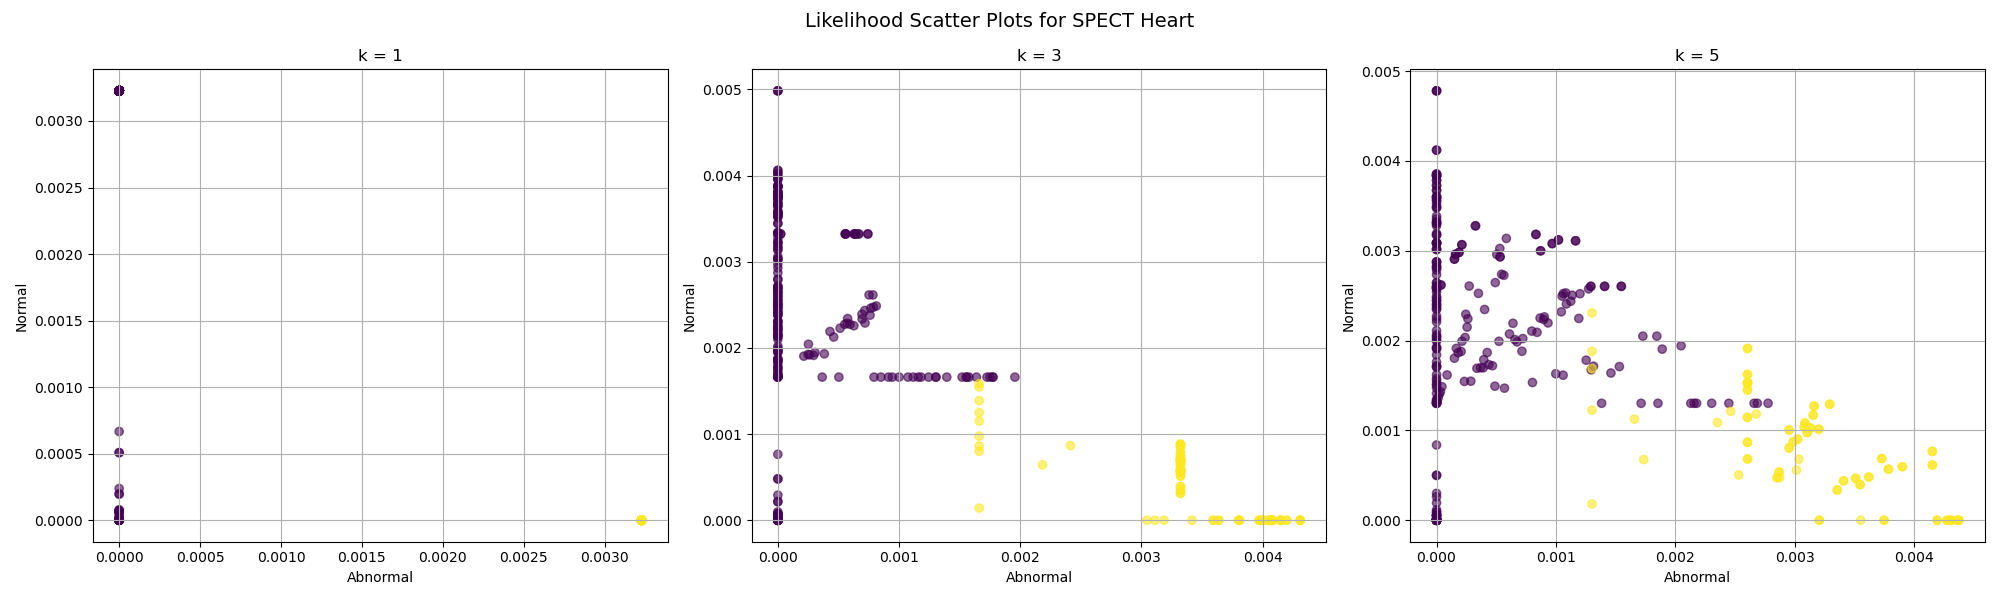
\includegraphics[width=0.45\textwidth]{../scripts/comparison_results/SPECT Heart_likelihood.png}
    \caption{Likelihood comparison for the SPECT Heart dataset.}
    \label{fig:spect_heart_likelihood}
\end{figure}

\subsection{Likelihood Analysis}

The likelihood distributions for each dataset, as shown in Figures \ref{fig:banknote_likelihood} to \ref{fig:spect_heart_likelihood}, provide insights into the performance of the KNN classifier across different scenarios. Each plot represents the sum of weighted votes for class 0 (x-axis) and class 1 (y-axis), with each point corresponding to a sample. The following observations can be made:

\begin{itemize}
    \item \textbf{Clear Separation:} Datasets such as Banknote, Breast Cancer, and Binary Digits exhibit well-separated clusters along the axes. This indicates that the KNN classifier assigns high confidence to most samples, resulting in distinct class boundaries. These datasets are characterized by low class overlap and high separability, which aligns with the high accuracy observed in Table \ref{tab:accuracy}.

    \item \textbf{Moderate Overlap:} Datasets like Ionosphere, Pima Diabetes, and Sonar show moderate overlap between the two classes. While the clusters are still distinguishable, a significant number of points lie near the diagonal, indicating ambiguous classifications. This overlap may contribute to slightly lower accuracy compared to datasets with clear separation.

    \item \textbf{Significant Overlap:} Haberman and SPECT Heart datasets display substantial overlap, with many points concentrated near the diagonal. This suggests that the KNN classifier struggles to confidently assign class labels, likely due to inherent noise or feature overlap in the data. These datasets also exhibit lower accuracy and higher ambiguity in classification.

    \item \textbf{Outliers:} Some datasets, such as Sonar and Ionosphere, contain outliers far from the main clusters. These points may correspond to misclassified or hard-to-classify samples, which could impact the overall performance of the classifier.

\end{itemize}

The likelihood analysis highlights the strengths and limitations of the KNN-CLAS method. Datasets with well-separated classes benefit from the simplicity and efficiency of KNN-CLAS, while those with significant overlap or noise present greater challenges. These findings emphasize the importance of dataset characteristics, such as class separability and feature overlap, in determining the effectiveness of the proposed method.

\section{Discussion}

The results confirm that KNN-CLAS effectively replaces NN-CLAS's filtering step with a Gabriel Graph (GG)-based support edge selection and KNN voting mechanism. While both methods utilize Gabriel Graphs, KNN-CLAS avoids vertex pruning by relying on inter-class edges and multi-neighbor consensus. This approach reduces training time by up to 82\% (e.g., Banknote dataset) but increases memory usage due to larger support sets.

KNN-CLAS demonstrates robustness to class imbalance (e.g., Haberman, Imbalance Ratio = 2.78) by relying on boundary-proximate support edges, which are less affected by skewed distributions. However, the increased number of support samples may pose challenges for memory-constrained systems.

Compared to NN-CLAS, which relies on computationally expensive filtering, KNN-CLAS achieves similar accuracy with significantly reduced training times. This makes it a practical alternative, particularly for resource-constrained environments.

The performance of KNN-CLAS is influenced by dataset characteristics such as class imbalance and feature overlap. For instance, in datasets with high imbalance ratios (e.g., Haberman), KNN-CLAS maintains competitive accuracy, showcasing its robustness.

\section{Future Work}
Future research could explore hybrid strategies that combine the strengths of NN-CLAS and KNN-CLAS. For example, selective filtering could minimize the number of support samples while maintaining computational efficiency. Additionally, enhancing KNN-CLAS for datasets with significant class overlap could involve techniques like feature selection, dimensionality reduction, or adaptive weighting schemes to improve class separability and classification performance.

\begin{thebibliography}{00}
    % reference papers
    \bibitem{torres2016} L. C. B. Torres, "Classificador por arestas de suporte (CLAS): métodos de aprendizado baseados em Grafos de Gabriel," Manuscript, 2016.
    \bibitem{souza2019} A. C. Souza, C. Leite Castro, J. A. Garcia, L. C. B. Torres, L. J. Acevedo Jaimes and B. R. A. Jaimes, "Improving the Efficiency of Gabriel Graph-based Classifiers for Hardware-optimized Implementations," 2019 XXII Symposium on Image, Signal Processing and Artificial Vision (STSIVA), Bucaramanga, Colombia, 2019.
    \bibitem{arias2021} J. Arias-Garcia et al., "Enhancing Performance of Gabriel Graph-Based Classifiers by a Hardware Co-Processor for Embedded System Applications," in IEEE Transactions on Industrial Informatics, vol. 17, no. 2, Feb. 2021.
    \bibitem{arias2024} J. Arias-Garcia et al., "Improved Design for Hardware Implementation of Graph-Based Large Margin Classifiers for Embedded Edge Computing," in IEEE Transactions on Neural Networks and Learning Systems, vol. 35, no. 1, Jan. 2024.
    \bibitem{torres2015} L. C. B. Torres, C. L. Castro and A. P. Braga, "A parameterless mixture model for large margin classification," 2015 International Joint Conference on Neural Networks (IJCNN), Killarney, Ireland, 2015.
    \bibitem{torres2021} L. C. B. Torres, C. L. Castro, F. Coelho and A. P. Braga, "Large Margin Gaussian Mixture Classifier With a Gabriel Graph Geometric Representation of Data Set Structure," in IEEE Transactions on Neural Networks and Learning Systems, vol. 32, no. 3, March 2021.
    \bibitem{torres2015b} L. C. B. Torres, C. L. Castro, F. Coelho, F. Sill Torres and A. P. Braga, "Distance-based large margin classifier suitable for integrated circuit implementation," Manuscript, 2015.

    % datasets
    \bibitem{uci_breast_cancer} D. Dua and C. Graff, "Breast Cancer Wisconsin (Diagnostic) Data Set," UCI Machine Learning Repository, 1995. [Online]. Available: \url{https://archive.ics.uci.edu/ml/datasets/Breast+Cancer+Wisconsin+(Diagnostic)}
    \bibitem{pima_diabetes} J. Brownlee, "Pima Indians Diabetes Dataset," GitHub Repository, 2020. [Online]. Available: \url{https://github.com/jbrownlee/Datasets}
    \bibitem{uci_haberman} D. Dua and C. Graff, "Haberman's Survival Data Set," UCI Machine Learning Repository, 1995. [Online]. Available: \url{https://archive.ics.uci.edu/ml/datasets/Haberman's+Survival}
    \bibitem{uci_banknote} D. Dua and C. Graff, "Data Banknote Authentication Data Set," UCI Machine Learning Repository, 1995. [Online]. Available: \url{https://archive.ics.uci.edu/ml/datasets/banknote+authentication}
    \bibitem{uci_sonar} D. Dua and C. Graff, "Connectionist Bench (Sonar, Mines vs. Rocks) Data Set," UCI Machine Learning Repository, 1995. [Online]. Available: \url{https://archive.ics.uci.edu/ml/datasets/connectionist+bench+(sonar,+mines+vs.+rocks)}
    \bibitem{uci_adult} D. Dua and C. Graff, "Adult Data Set," UCI Machine Learning Repository, 1995. [Online]. Available: \url{https://archive.ics.uci.edu/ml/datasets/adult}
    \bibitem{uci_ionosphere} D. Dua and C. Graff, "Ionosphere Data Set," UCI Machine Learning Repository, 1995. [Online]. Available: \url{https://archive.ics.uci.edu/ml/datasets/ionosphere}
    \bibitem{uci_spect_heart} D. Dua and C. Graff, "SPECT Heart Data Set," UCI Machine Learning Repository, 1995. [Online]. Available: \url{https://archive.ics.uci.edu/ml/datasets/SPECT+Heart}
    \bibitem{sklearn_digits} L. Breiman et al., "Optical Recognition of Handwritten Digits Data Set," Scikit-learn Documentation, 1998. [Online]. Available: \url{https://scikit-learn.org/stable/modules/generated/sklearn.datasets.load_digits.html}
\end{thebibliography}

\end{document}
